\documentclass[main.tex]{subfile}

\section{Graphs} 
\label{sec:graphs}

\begin{figure}[H]
	\includegraphics[width=\textwidth]{step.png}
	\caption{Step Responses of $G_1$ - $G_4$}
\end{figure}

\begin{figure}[H]
	\includegraphics[width=\textwidth]{g3sim.png}
	\caption{$G_3$ Simulation}
\end{figure}

\begin{figure}[H]
	\includegraphics[width=\textwidth]{g1sim.png}
	\caption{$G_1$ Simulation}
\end{figure}

\begin{figure}[H]
	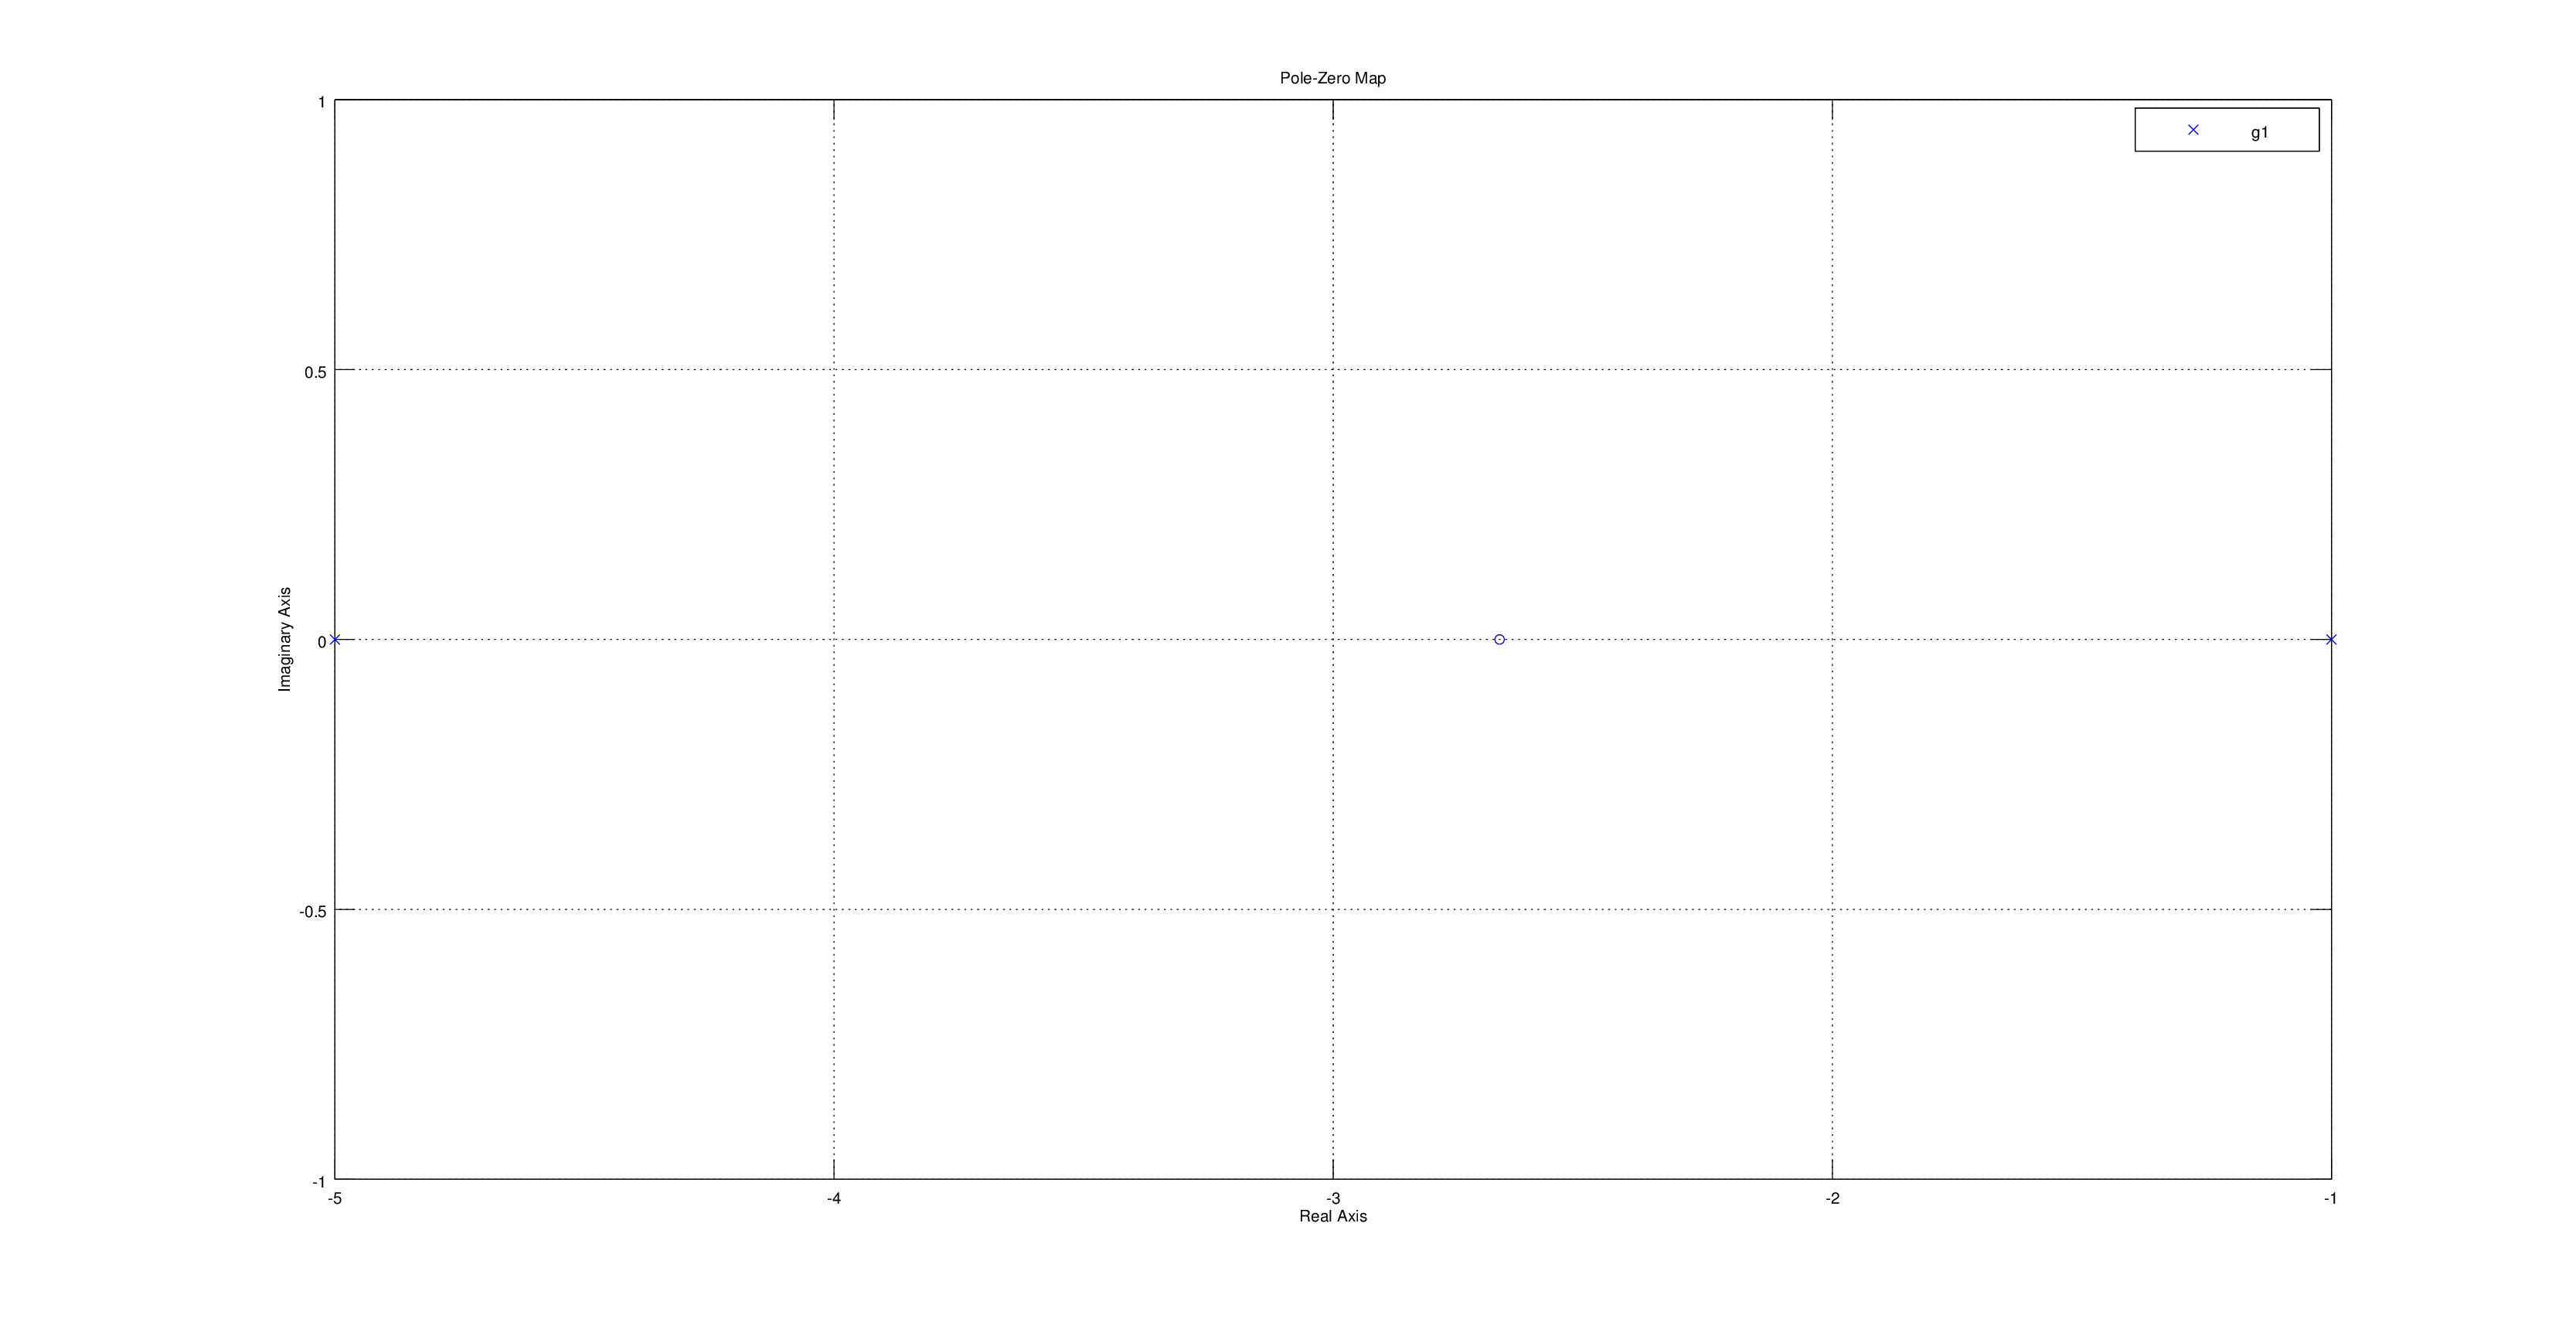
\includegraphics[width=\textwidth]{g1.png}
	\caption{$\mathrm{G}_1$ Pole-Zero Graph}
\end{figure}
\begin{figure}[H]
	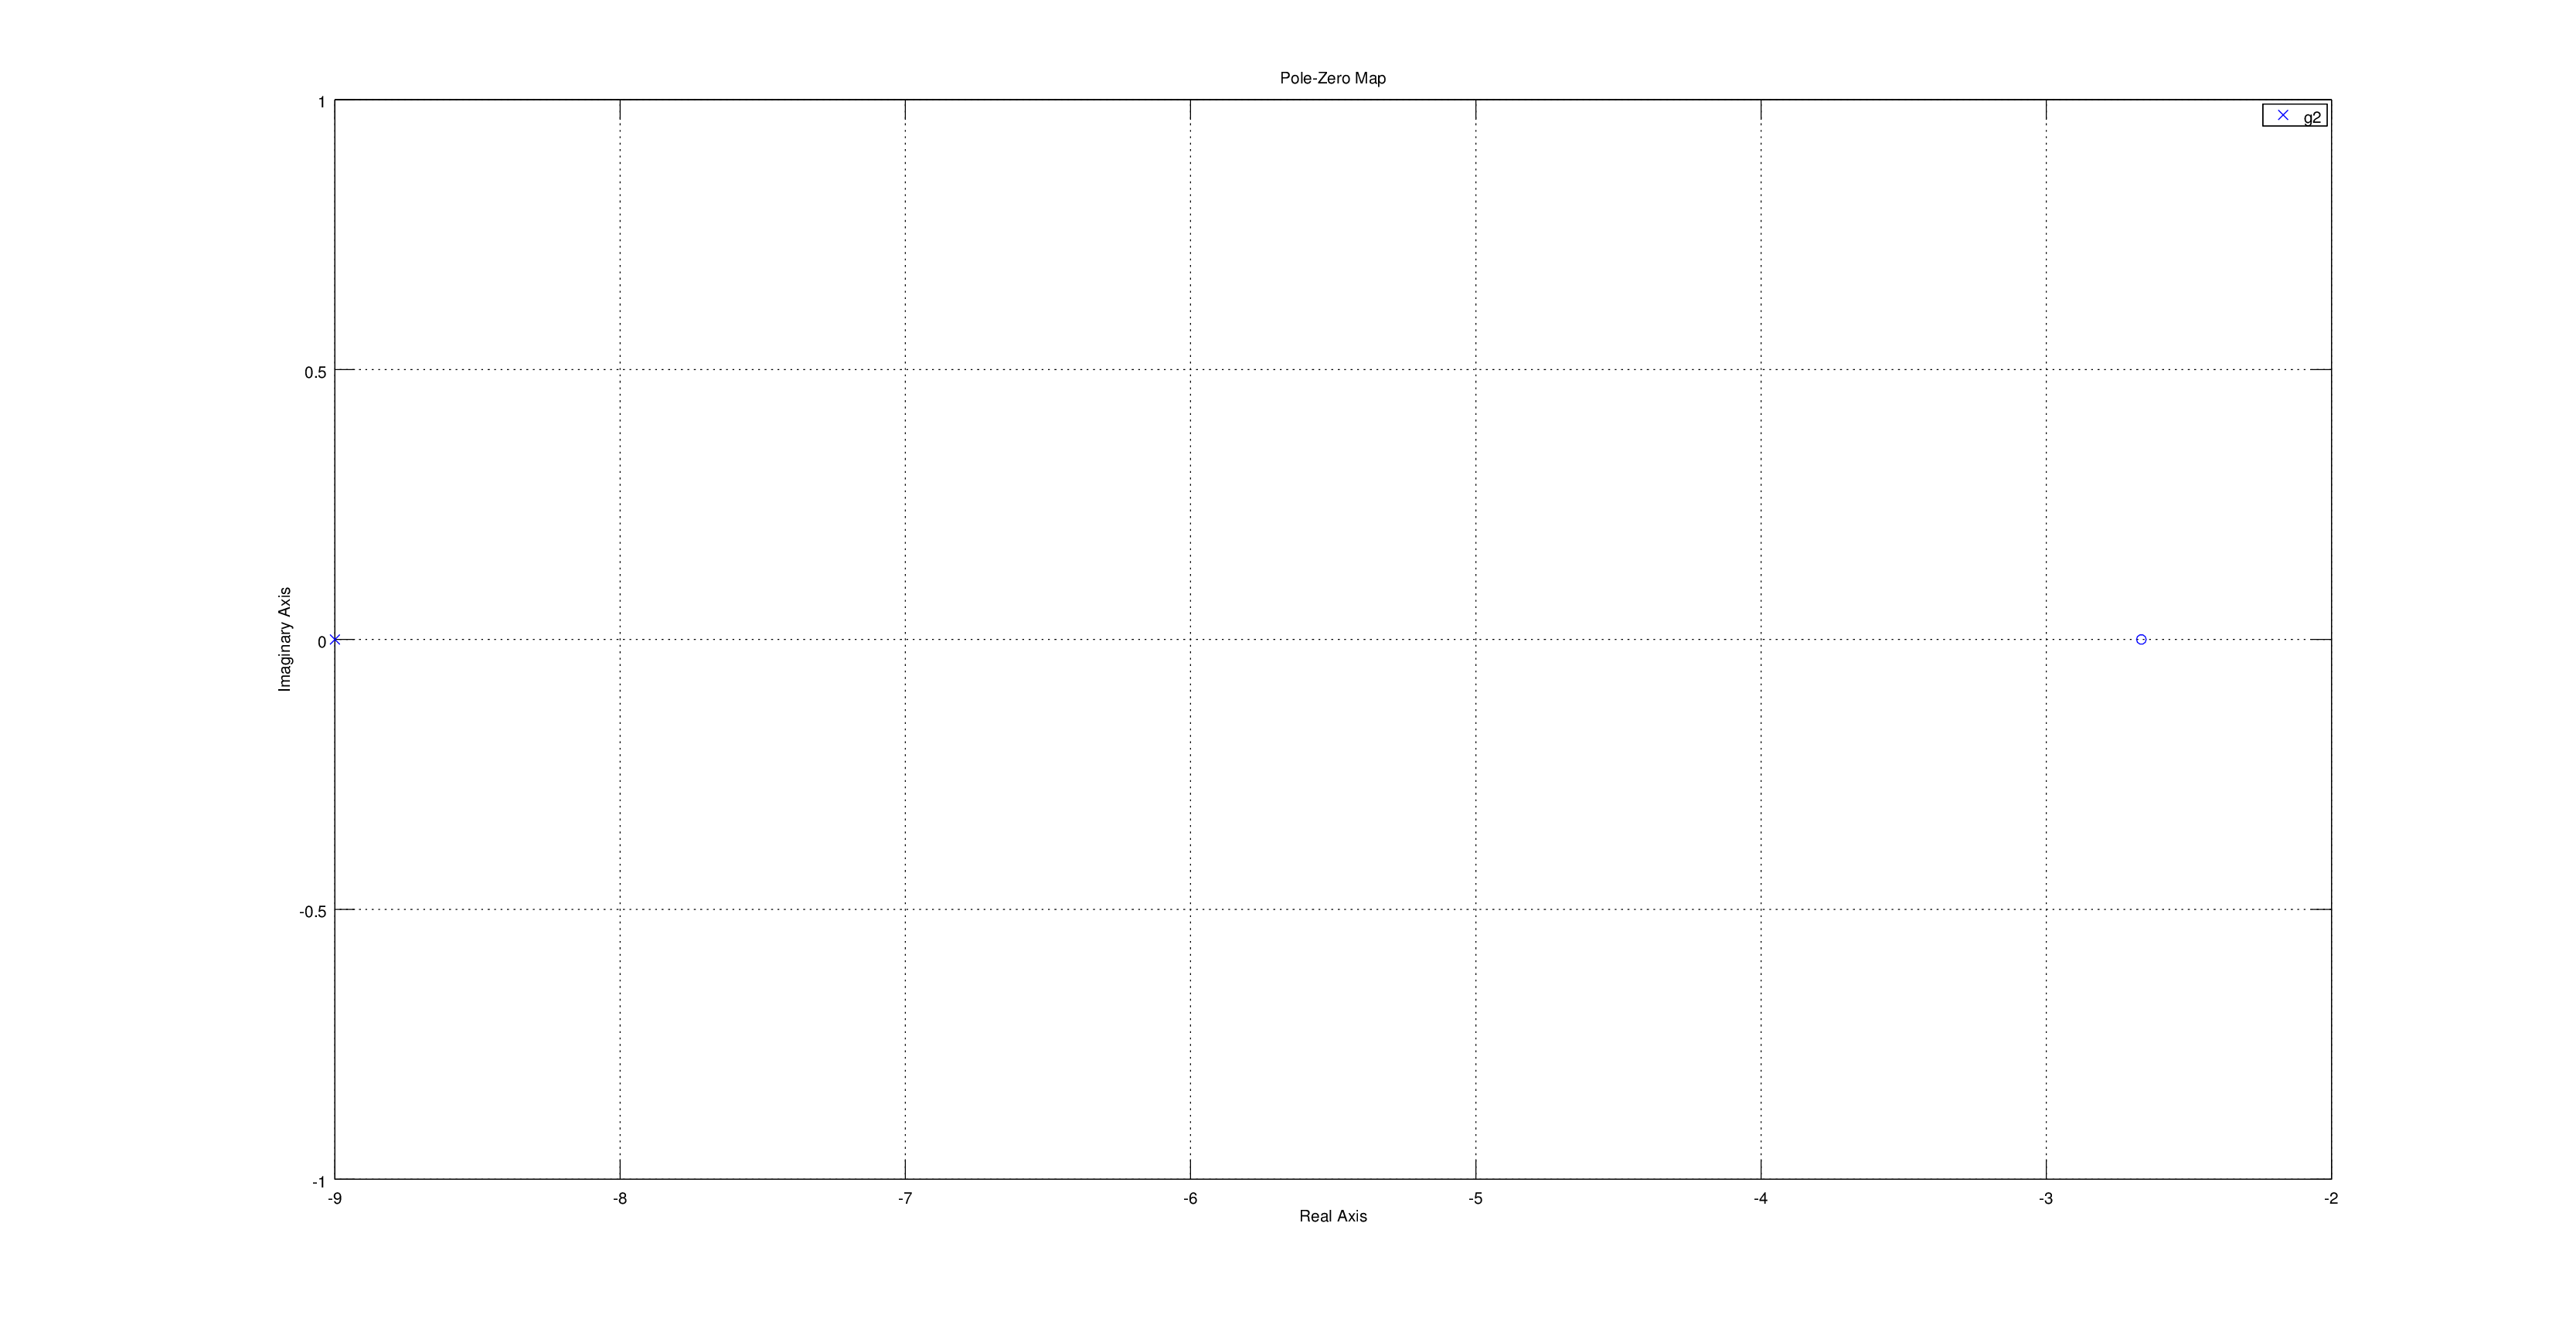
\includegraphics[width=\textwidth]{g2.png}
	\caption{$\mathrm{G}_2$ Pole-Zero Graph}
\end{figure}

\begin{figure}[H]
	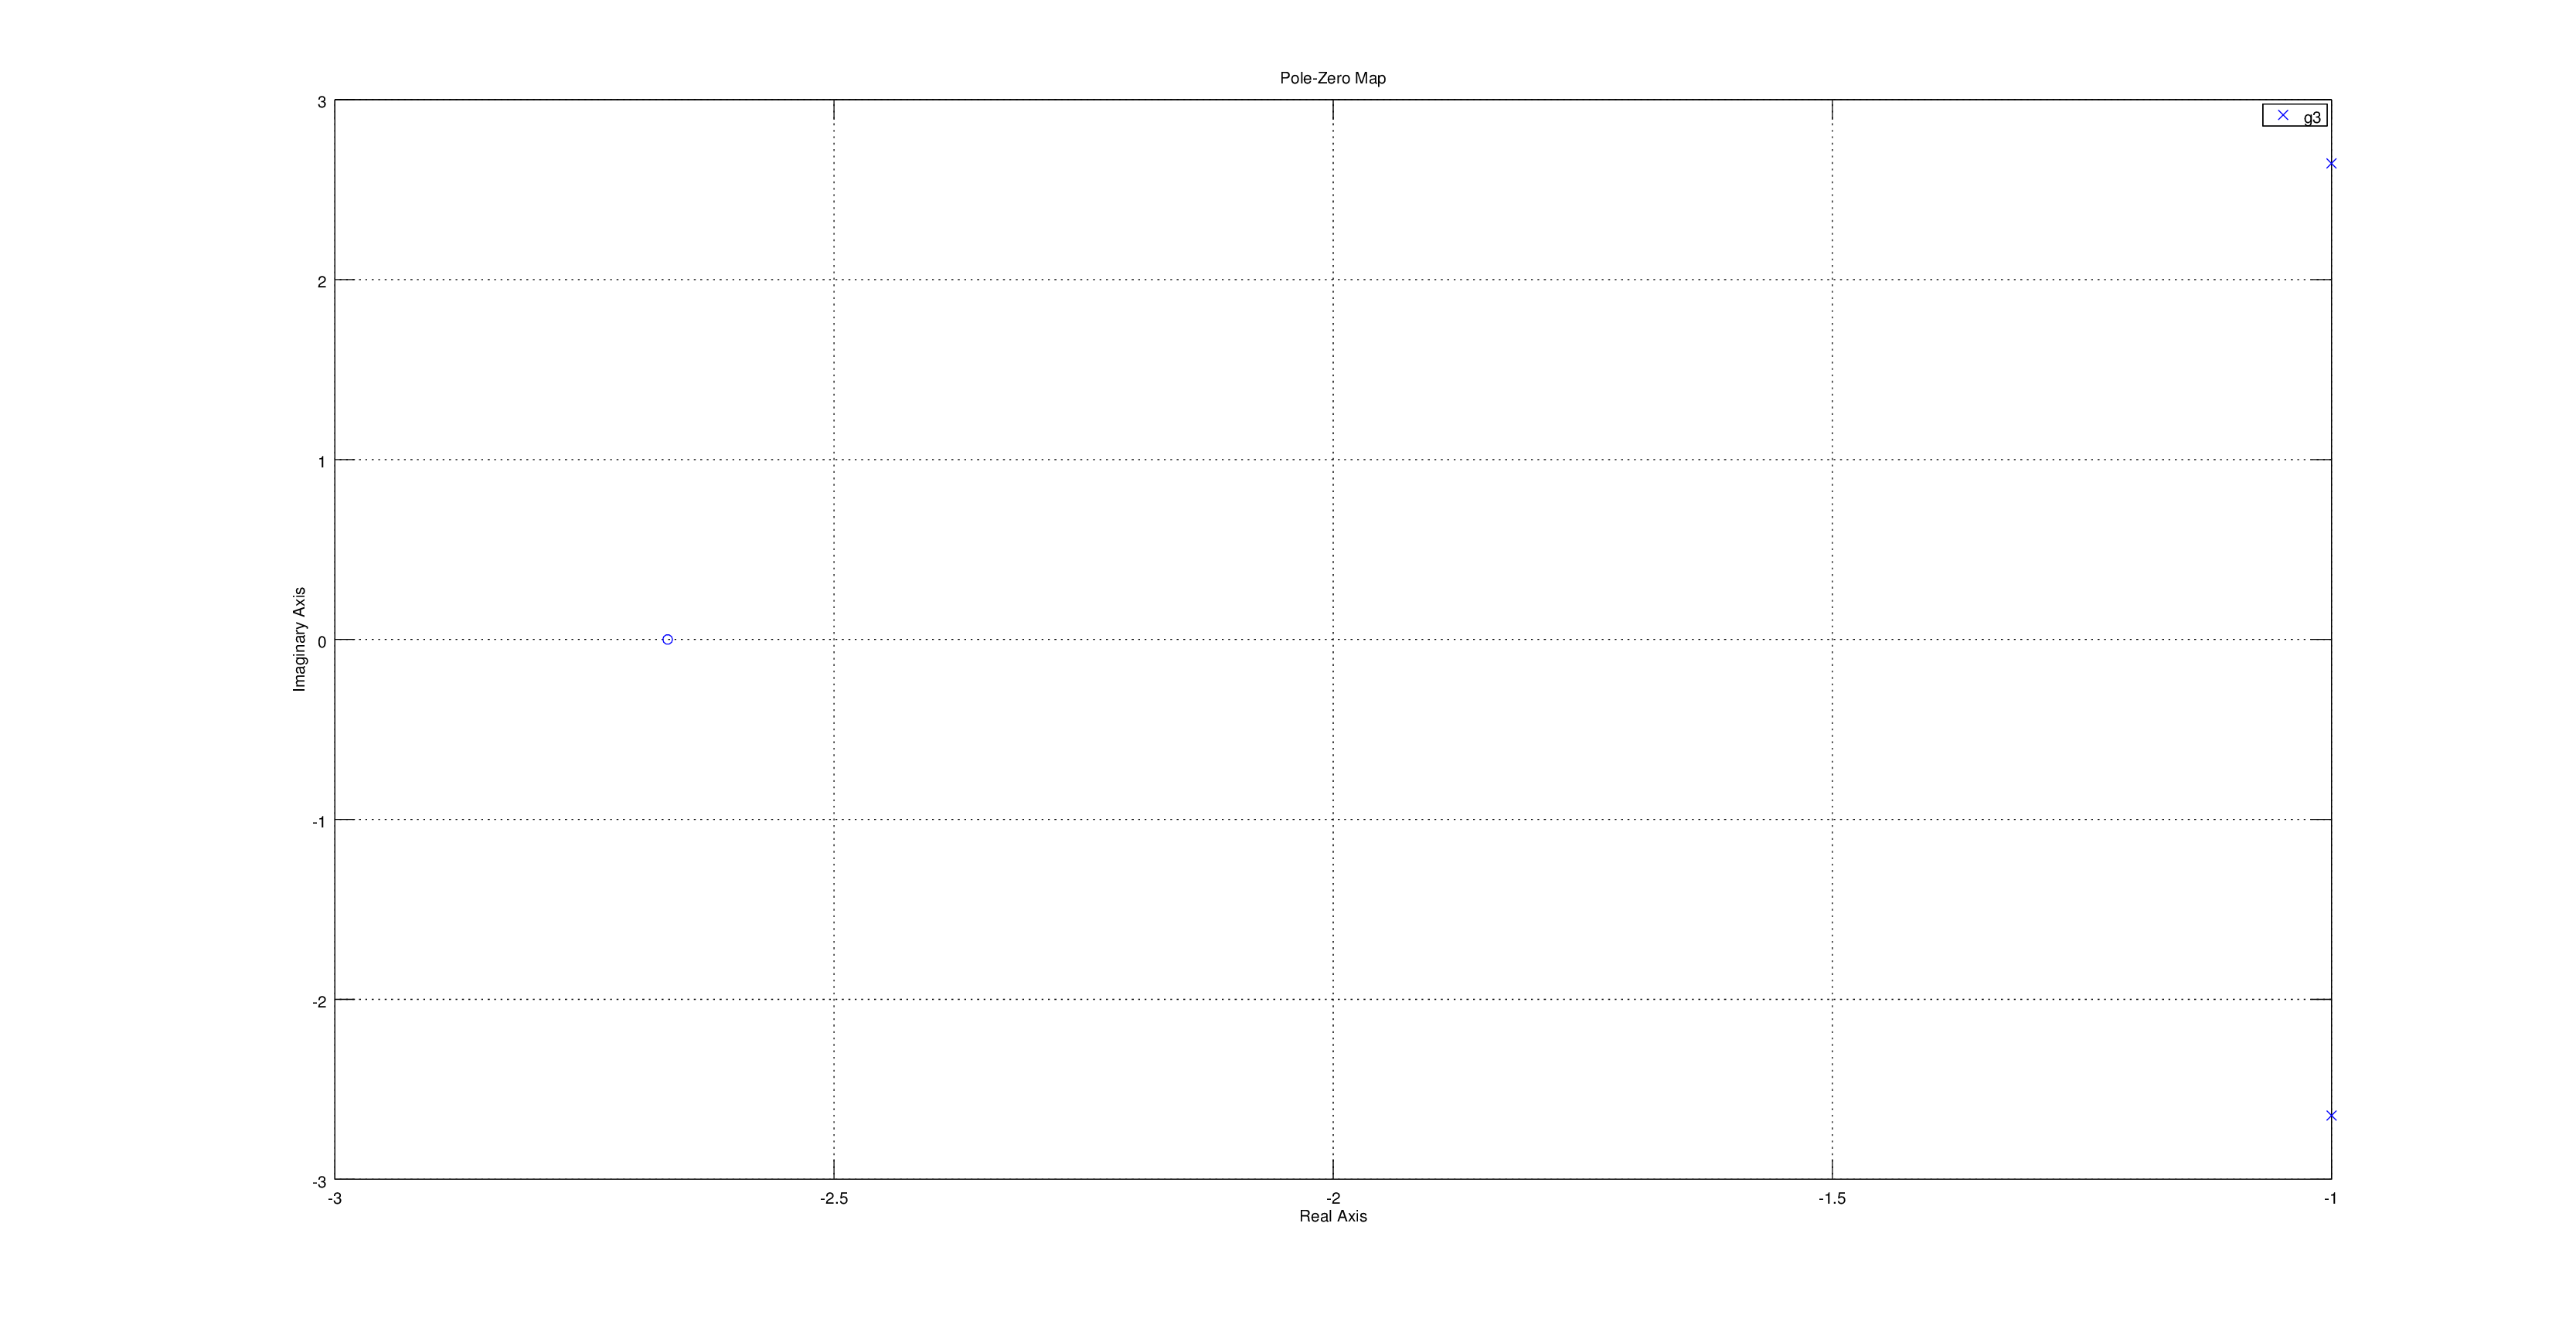
\includegraphics[width=\textwidth]{g3.png}
	\caption{$\mathrm{G}_3$ Pole-Zero Graph}
\end{figure}

\begin{figure}[H]
	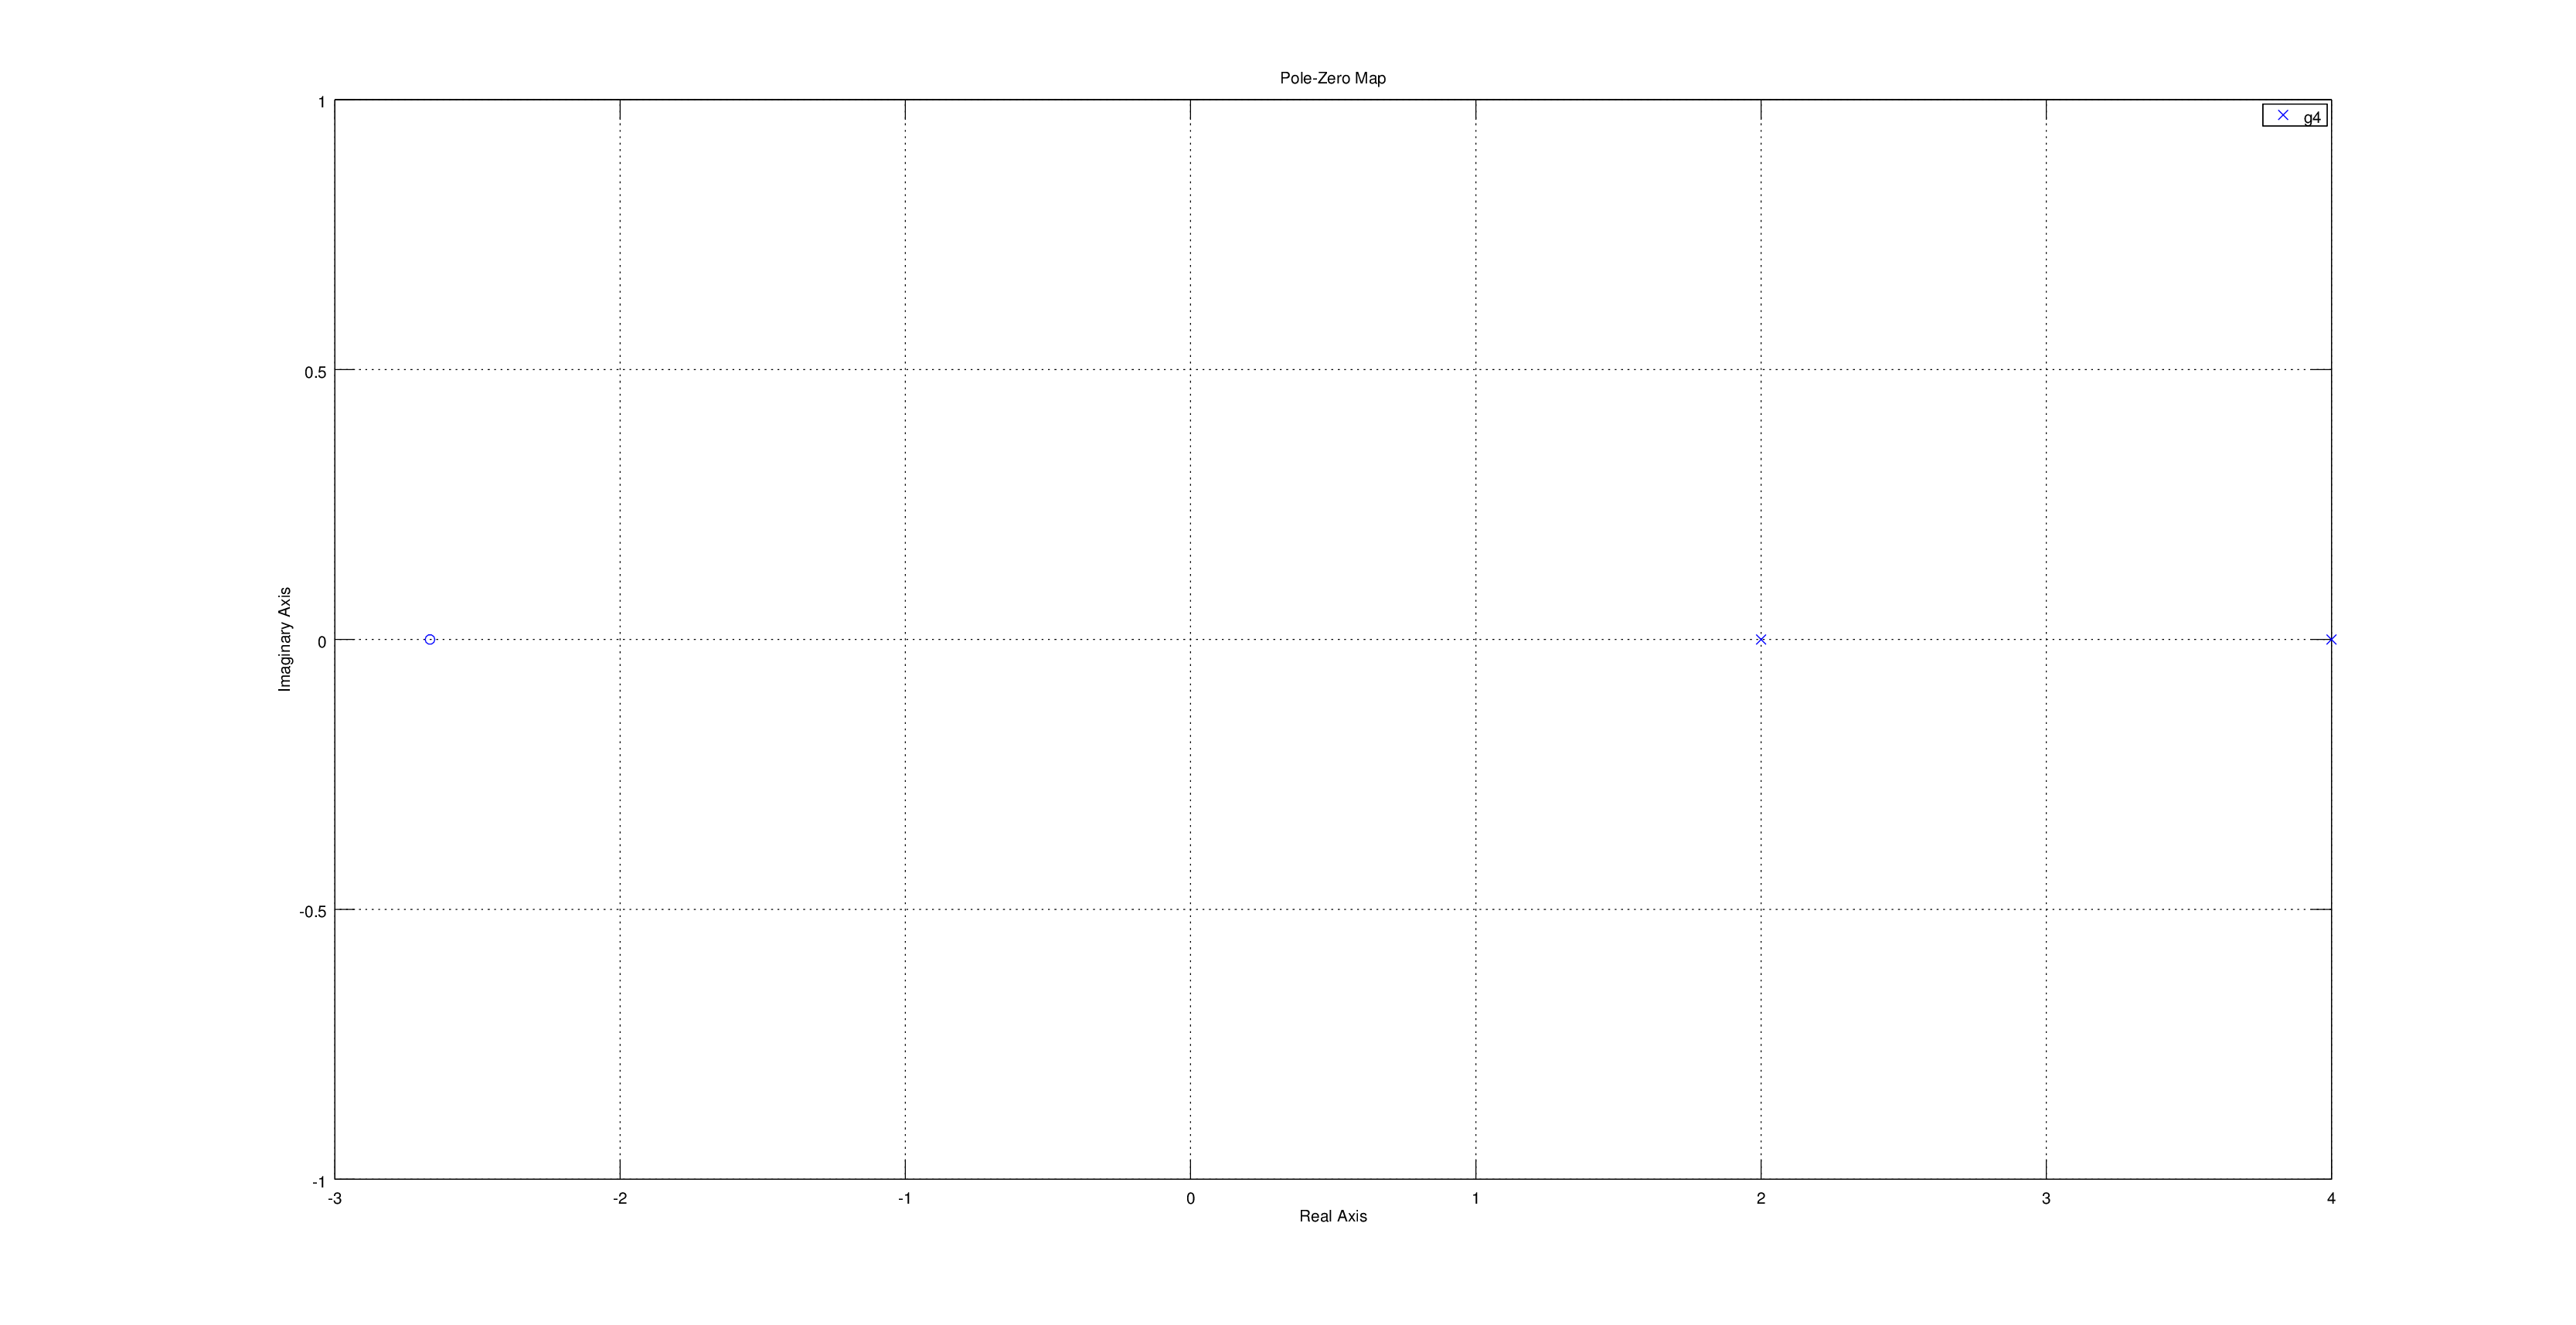
\includegraphics[width=\textwidth]{g4.png}
	\caption{$\mathrm{G}_4$ Pole-Zero Graph}
\end{figure}

\subsection{Simulink Results}

\label{sub:simulink_results}
\begin{figure}[H]
	\includegraphics[width=\textwidth]{g3simlinkmodel.png}
	\caption{$\mathrm{G}_3$ Simulink Model}
\end{figure}
\begin{figure}[H]
	\includegraphics[width=\textwidth]{g3simlinkgraph.png}
	\caption{$\mathrm{G}_3$ Simulink Results}
\end{figure}

% subsection simulink_results (end)

% section graphs (end)

\section{Source Code} 
\label{sec:source_code}

\lstinputlisting[language=octave,title=lab1.m]{src/main.m}

\section{Output} 
\label{sec:output}

\lstinputlisting[language=tcl,title=main.out]{src/main_out.txt}

% section output (end)

% section source_code (end)
